%%%%%%%%%%%%%%%%%%%%%%%%%%%%%%%%%%%%%%%%%%%%%%%%%%%%%%%%%%%
\begin{frame}
  \begin{center}
    {\Large Phishing Detection using NLP}
	
	\tiny{(Ref: Using machine learning for phishing domain detection By Prasad Ramesh)}
  \end{center}
\end{frame}

%%%%%%%%%%%%%%%%%%%%%%%%%%%%%%%%%%%%%%%%%%%%%%%%%%%%%%%%%%%
\begin{frame}[fragile]\frametitle{Applications of Deep Learning}
	\begin{itemize}
	\item  Attackers use disguised email addresses as a weapon to target large companies. 
	\item With the huge number of phishing emails received every day, companies are not able to detect all of them. 
	\item Here, we will build machine learning models to detect phishing attempts, using Python.
	\end{itemize}
\end{frame}

%%%%%%%%%%%%%%%%%%%%%%%%%%%%%%%%%%%%%%%%%%%%%%%%%%%%%%%%%%%
\begin{frame}
  \begin{center}
    {\Large Data}
  \end{center}
\end{frame}


%%%%%%%%%%%%%%%%%%%%%%%%%%%%%%%%%%%%%%%%%%%%%%%%%%%%%%%%%%%
\begin{frame}[fragile]\frametitle{Data}
Data : https://archive.ics.uci.edu/ml/datasets/Phishing+Websites

	    \begin{center}
     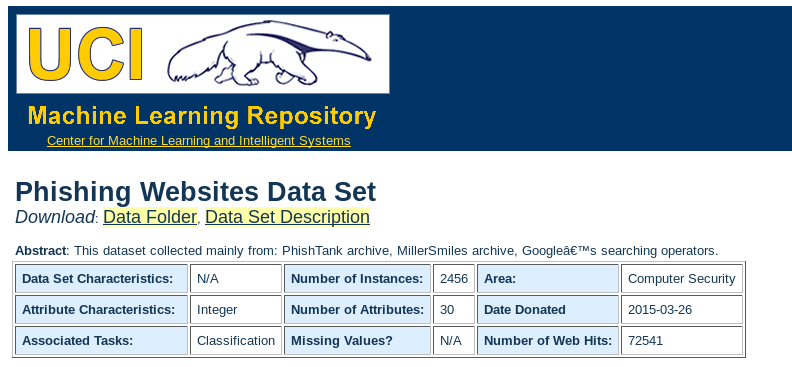
\includegraphics[width=0.8\linewidth]{secdnlp2}      
     \end{center}
\end{frame}

%%%%%%%%%%%%%%%%%%%%%%%%%%%%%%%%%%%%%%%%%%%%%%%%%%%%%%%%%%%
\begin{frame}[fragile]\frametitle{Data}
The dataset is provided as an arff file:

	    \begin{center}
     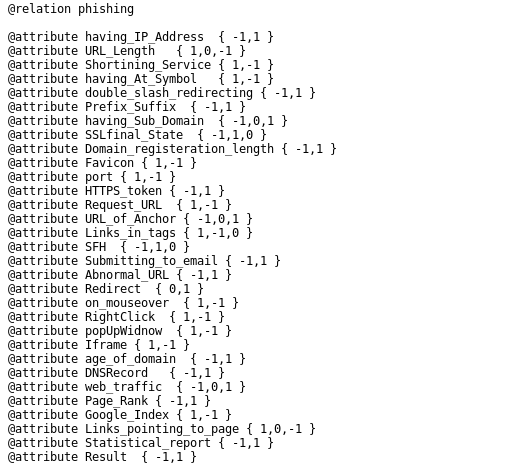
\includegraphics[width=0.5\linewidth]{secdnlp3}      
     \end{center}
\end{frame}

%%%%%%%%%%%%%%%%%%%%%%%%%%%%%%%%%%%%%%%%%%%%%%%%%%%%%%%%%%%
\begin{frame}[fragile]\frametitle{Data}
The following is a snapshot from the dataset:
	    \begin{center}
     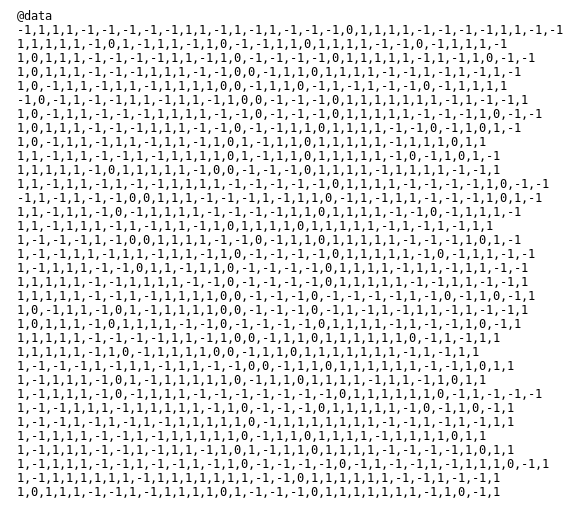
\includegraphics[width=0.5\linewidth]{secdnlp4}      
     \end{center}
\end{frame}

%%%%%%%%%%%%%%%%%%%%%%%%%%%%%%%%%%%%%%%%%%%%%%%%%%%%%%%%%%%
\begin{frame}[fragile]\frametitle{Data}
For better manipulation, we have organized the dataset into a csv file:
	    \begin{center}
     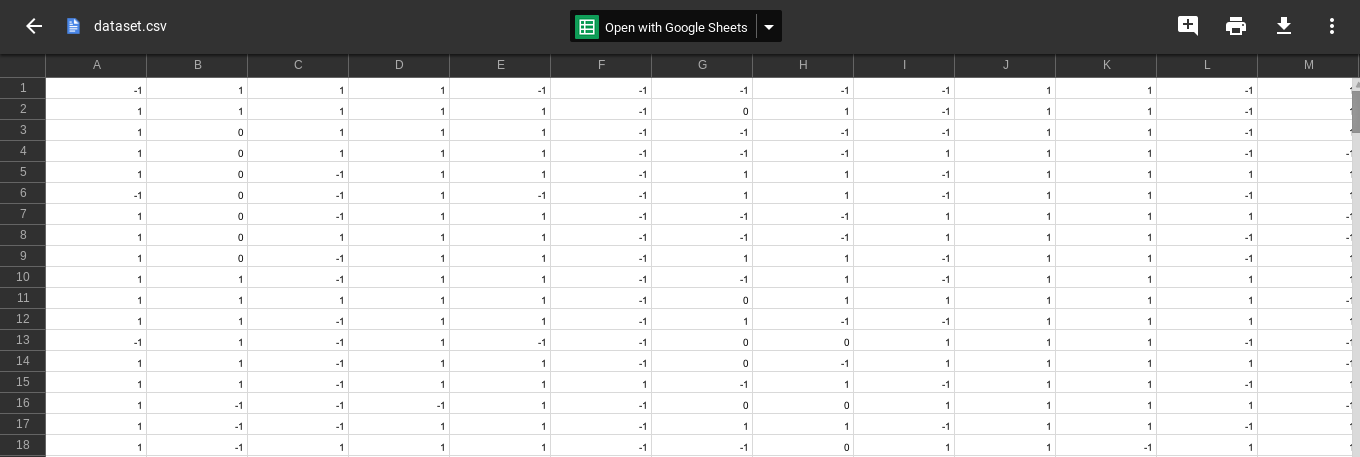
\includegraphics[width=\linewidth]{secdnlp5}      
     \end{center}
\end{frame}

%%%%%%%%%%%%%%%%%%%%%%%%%%%%%%%%%%%%%%%%%%%%%%%%%%%%%%%%%%%
\begin{frame}[fragile]\frametitle{Data}
Each line of the dataset is represented in the following format – \{30 Attributes (having\_IP\_Address URL\_Length, abnormal\_URL and so on)\} + \{1 Attribute (Result)\}:

	    \begin{center}
     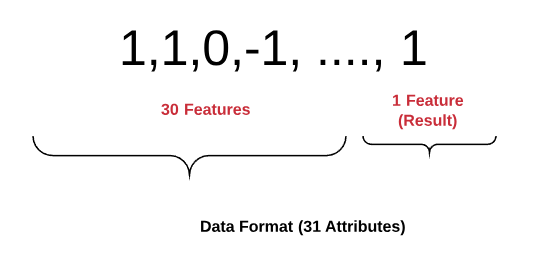
\includegraphics[width=0.5\linewidth]{secdnlp6}      
     \end{center}
\end{frame}

%%%%%%%%%%%%%%%%%%%%%%%%%%%%%%%%%%%%%%%%%%%%%%%%%%%%%%%%%%%
\begin{frame}
  \begin{center}
    {\Large Implementation}
  \end{center}
\end{frame}

%%%%%%%%%%%%%%%%%%%%%%%%%%%%%%%%%%%%%%%%%%%%%%%%%%%%%%%%%%%
\begin{frame}[fragile]\frametitle{Load Libraries and Data}
\begin{lstlisting}
import numpy as np
from sklearn import *
from sklearn.linear_model import LogisticRegression
from sklearn.metrics import accuracy_score

training_data = np.genfromtxt('dataset.csv', delimiter=',', dtype=np.int32)
\end{lstlisting}
\end{frame}

%%%%%%%%%%%%%%%%%%%%%%%%%%%%%%%%%%%%%%%%%%%%%%%%%%%%%%%%%%%
\begin{frame}[fragile]\frametitle{Prepare Training Data}

Identify the inputs (all of the attributes, except for the last one) and the outputs (the last attribute):

\begin{lstlisting}
inputs = training_data[:,:-1]
outputs = training_data[:, -1]

training_inputs = inputs[:2000]
training_outputs = outputs[:2000] 
testing_inputs = inputs[2000:]
testing_outputs = outputs[2000:]
\end{lstlisting}
\end{frame}

%%%%%%%%%%%%%%%%%%%%%%%%%%%%%%%%%%%%%%%%%%%%%%%%%%%%%%%%%%%
\begin{frame}[fragile]\frametitle{Modeling}

\begin{lstlisting}
classifier = LogisticRegression()
classifier.fit(training_inputs, training_outputs)
predictions = classifier.predict(testing_inputs)
accuracy = 100.0 * accuracy_score(testing_outputs, predictions)

print ("The accuracy of your Logistic Regression on testing data is: " + str(accuracy))

>> 84.85
\end{lstlisting}

The accuracy of our model is approximately 85\%. This is a good accuracy, since our model detected 85 phishing URLs out of 100. 
\end{frame}